\chapter{Wheat Diseases and Insect Pests – Challenges, Impacts, and Smart Agriculture Solutions}

\section{Introduction}

Wheat is a crucial global crop, but its production is threatened by various diseases and insect pests, leading to significant yield losses. Traditional detection and control methods are often ineffective, highlighting the need for improved solutions. 

This chapter explores common wheat diseases and pests, their impact on agriculture, and the importance of timely detection. It also discusses strategies for enhancing disease control and the challenges of implementing smart agricultural technologies.



\section{The Motivation to Protect Wheat}

Wheat is an ancient and vital food crop that provides energy and feeds billions of people around the world (see Figure~\ref{fig:Figure01}). Its demand is growing quickly because it’s used in many affordable food products and plays a big role in global food security. The FAO (Food and Agriculture Organization) estimates that by 2050, the world will need about 840 million tonnes of wheat, up from 642 million tonnes today \parencite{sharma2015wheat}. This doesn’t even include the extra needs like animal feed or the impact of climate change.

To meet this growing demand, developing countries need to increase wheat production by 77\%, mostly by improving how much wheat is grown on the same land \parencite{sharma2015wheat}. But this is becoming harder, as wheat productivity is slowing down and diseases are becoming a bigger problem. If we don’t manage pests and diseases properly, wheat production could fall short of what the world needs.

That’s why it's important to invest in research, use better farming methods, and grow disease-resistant wheat. Protecting this essential crop is key to making sure we have enough food for the future.


\begin{figure}[H]
    \centering
    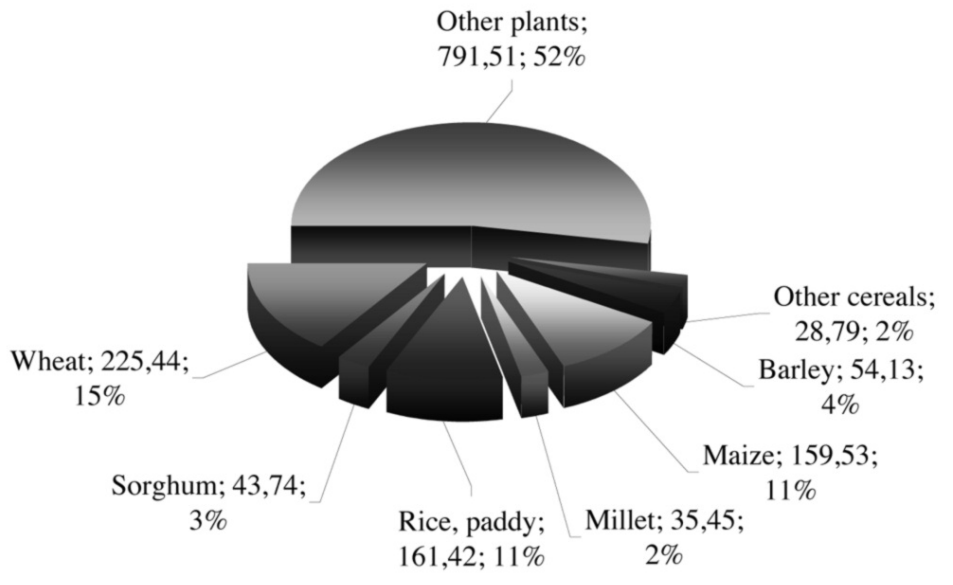
\includegraphics[width=0.7\textwidth]{chapters/chapter2/images/Figure01.png}
    \caption{Division of sowing area in the world in 2009 (in million hectares and percentage) Source: FAO, 2011}
    \label{fig:Figure01}
\end{figure}


\section{Wheat Diseases: Types and Impacts}

Wheat diseases caused by fungi are influenced by several factors, including plant resistance, spore density, temperature, and environmental conditions, especially the presence of moisture on plant surfaces, which facilitates infection. While some fungi are host-specific, others can infect a wide range of plants. Symptoms can differ greatly, making accurate identification essential. Researchers primarily rely on fungal morphology for diagnosis. A clear understanding of these diseases is key to effective management and control. The following classification (Figure ~\ref{fig:Figure02}) outlines the major wheat diseases, grouped by their causes and the plant parts they affect.

\begin{figure}[H]
    \centering
    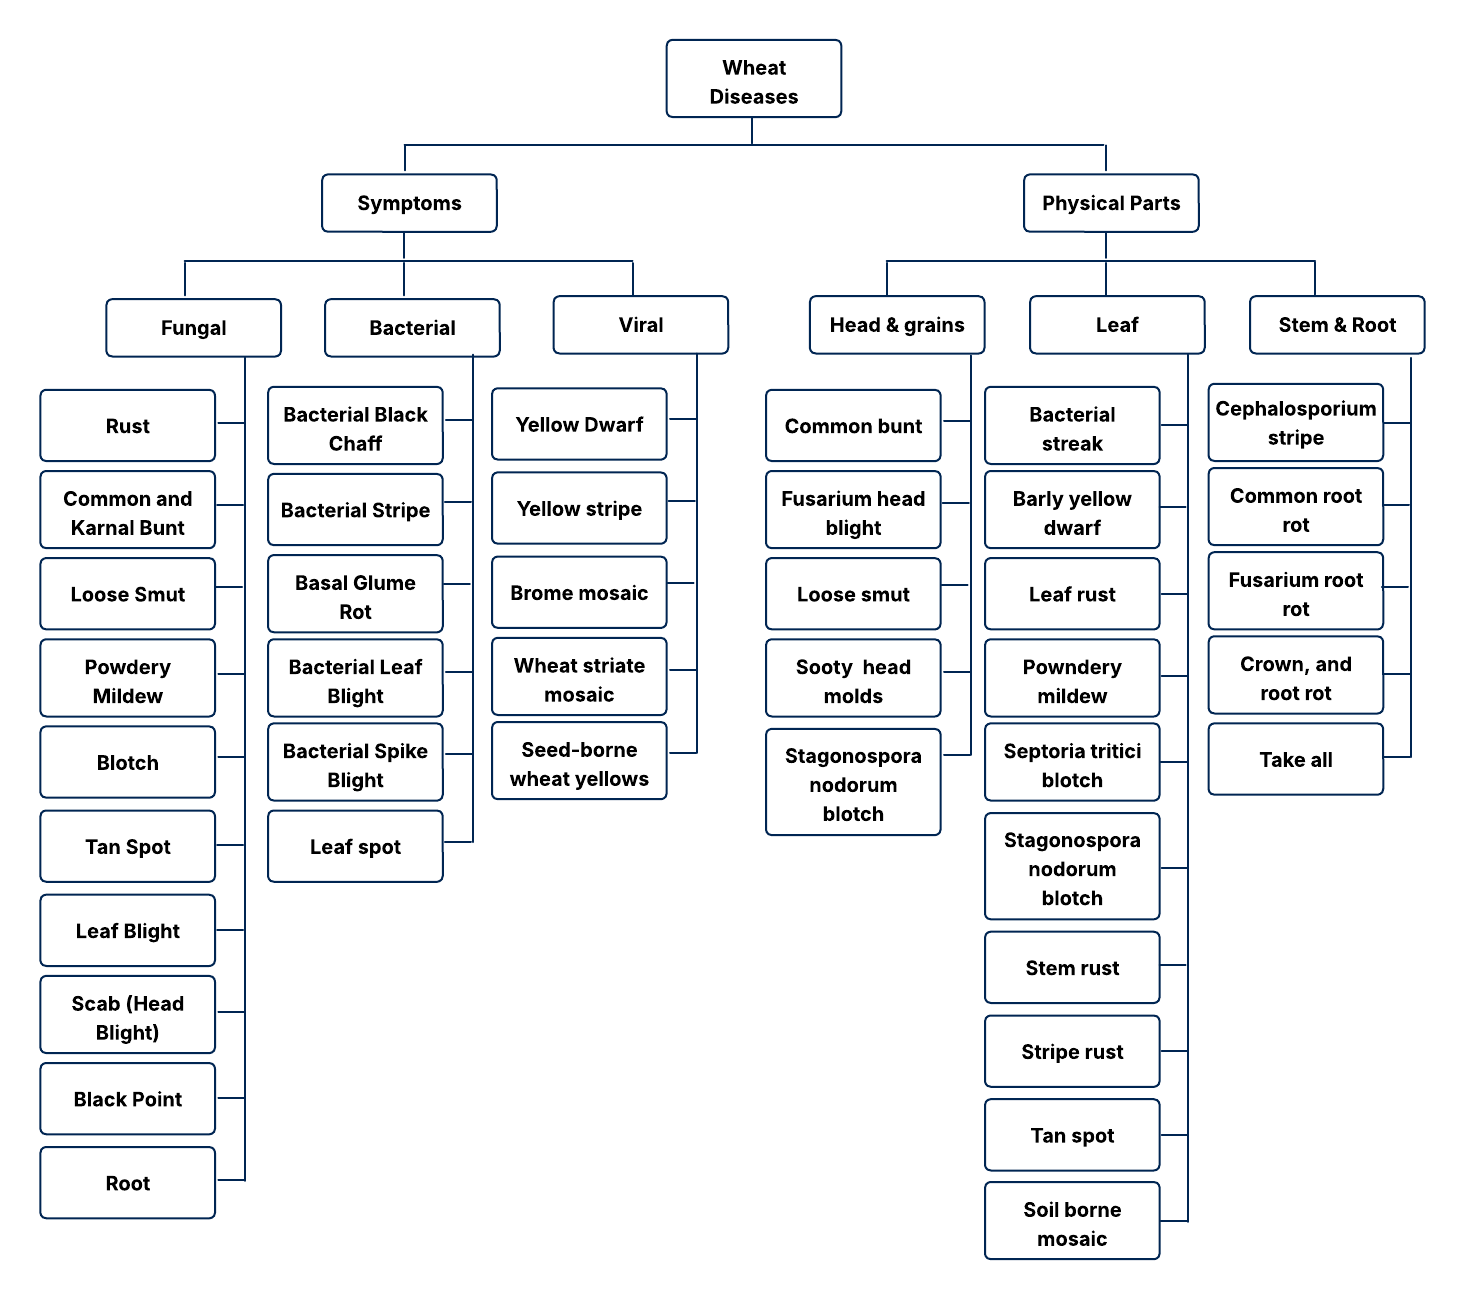
\includegraphics[width=0.8
    \textwidth]{chapters/chapter2/images/Figure02.png}
    \caption{Taxonomy of wheat diseases \protect\parencite{haider2021wheat}}
    \label{fig:Figure02}
\end{figure}

\subsection{Leaf Rust (Brown Rust)}  duveiller2012wheat

Leaf rust, caused by Puccinia triticina, appears as small, circular, orange to brown pustules on the upper surfaces of leaves and leaf sheaths. It spreads through wind-borne spores and develops quickly in moist conditions at around 20°C. New spores form every 10–14 days if conditions are favorable. As plants mature or conditions worsen, black spores may appear (as shown in Figure~\ref{fig:Figure03} ). This disease affects wheat, triticale, and related grasses and is common in temperate cereal-growing regions. Severe infections reduce grain yield, kernel number, weight, and quality \parencite{duveiller2012wheat}.  

\begin{figure}[H]
    \centering
    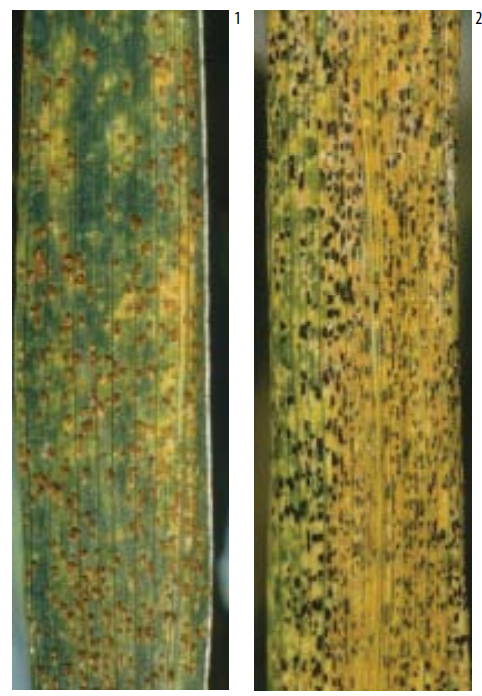
\includegraphics[width=0.2\textwidth]{chapters/chapter2/images/Figure03.png}
    \caption{Leaf rust with Brown spores (1), Leaf rust with Black spores(2) \protect\parencite{duveiller2012wheat}}
    \label{fig:Figure03}
\end{figure}

\subsection{Stem Rust (Black Rust)}
Stem rust, caused by Puccinia graminis, appears as dark reddish-brown pustules on leaves, stems, and spikes (as observed in Figure~\ref{fig:Figure04}). Light infections show scattered pustules, while severe cases cause them to merge. Before pustules form, small flecks may appear, and infected areas feel rough. The disease spreads through wind-borne spores and develops quickly in moist conditions with temperatures around 20°C. New spores can form in 10–15 days. It affects wheat, barley, triticale, and related grasses and is common in temperate cereal regions. Severe infections can reduce grain weight and quality and, in extreme cases, lead to total crop loss \parencite{duveiller2012wheat}.


\begin{figure}[H]
    \centering
    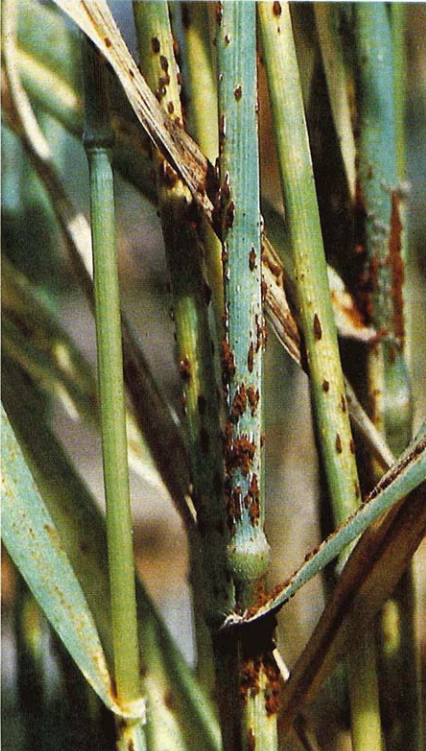
\includegraphics[width=0.2\textwidth]{chapters/chapter2/images/Figure04.png}
    \caption{Stem rust \protect\parencite{duveiller2012wheat}}
    \label{fig:Figure04}
\end{figure}

\subsection{Stripe Rust (Yellow Rust)}
 Stripe rust, caused by Puccinia striiformis, appears as yellow to orange-yellow pustules forming narrow stripes on leaves, leaf sheaths, necks, and glumes (as seen in Figure~\ref{fig:Figure05}). It spreads through wind-borne spores and develops quickly in moist conditions at temperatures between 10–20°C but slows down above 25°C. Severe infections reduce grain yield, kernel number, weight, and quality \parencite{duveiller2012wheat}.


\begin{figure}[H]
    \centering
    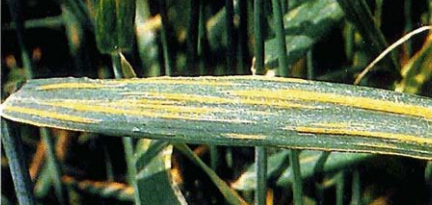
\includegraphics[width=0.5\textwidth]{chapters/chapter2/images/Figure05.png}
    \caption{Stripe rust \protect\parencite{duveiller2012wheat}}
    \label{fig:Figure05}
\end{figure}

\subsection{Blotch Diseases} 
The blotch diseases, which include Septoria tritici blotch (STB), Septoria nodorum blotch (SNB), and tan spot (TS) (as presented in Figure~\ref{fig:Figure06}), are caused by the Ascomycete fungi Zymoseptoria tritici, Parastagonospora nodorum, and Pyrenophora tritici-repentis, respectively \parencite{figueroa2018review}.


\begin{figure}[H]
    \centering
    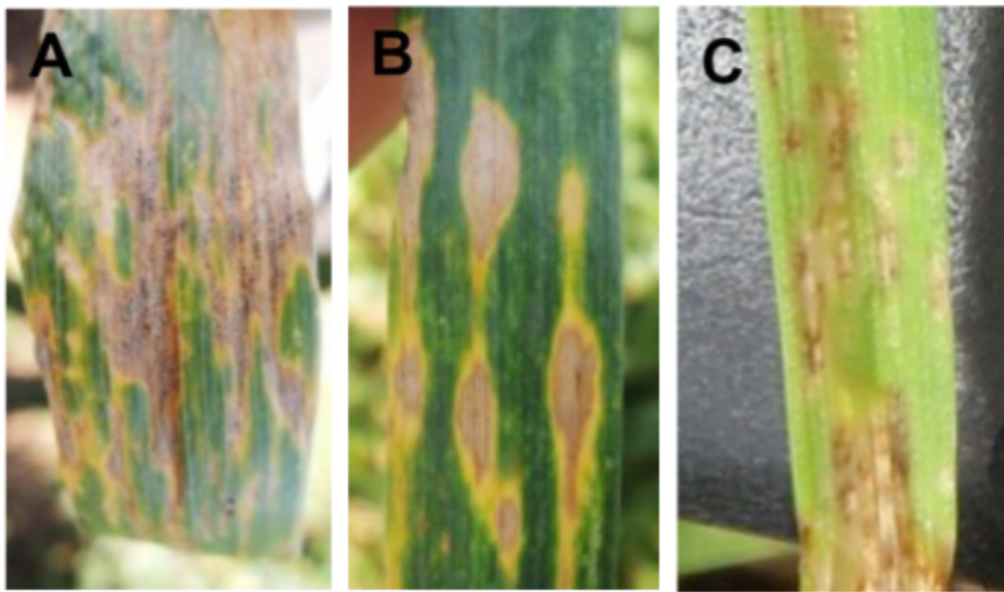
\includegraphics[width=0.5\textwidth]{chapters/chapter2/images/Figure06.png}
    \caption{Symptoms of foliar blotch diseases. (A) Septoria tritici blotch. (B) Tan spot. (C) Septoria nodorum blotch \protect\parencite{figueroa2018review}}
    \label{fig:Figure06}
\end{figure}

\subsection{Fusarium Head Blight (FHB)}
Fusarium head blight (FHB), also known as wheat scab or ear blight, is a major disease of wheat caused primarily by the Ascomycete fungus Fusarium graminearum (Fg). It can also be caused by other regional Fusarium species \parencite{figueroa2018review}.
Fusarium head blight appears as dark, oily florets with pinkish spores (as seen in Figure~\ref{fig:Figure07}). Infected kernels may be covered in white fungal growth. The disease spreads in warm, humid conditions (10–28°C), infecting spikes during flowering and spreading between florets. It affects all small grain cereals and is found in most soils and crop residues. Severe infections can reduce yields by over 50\%  and lower grain quality. Contaminated grain may contain harmful mycotoxins, making it unsafe for humans and animals \parencite{duveiller2012wheat}.

\begin{figure}[H]
    \centering
    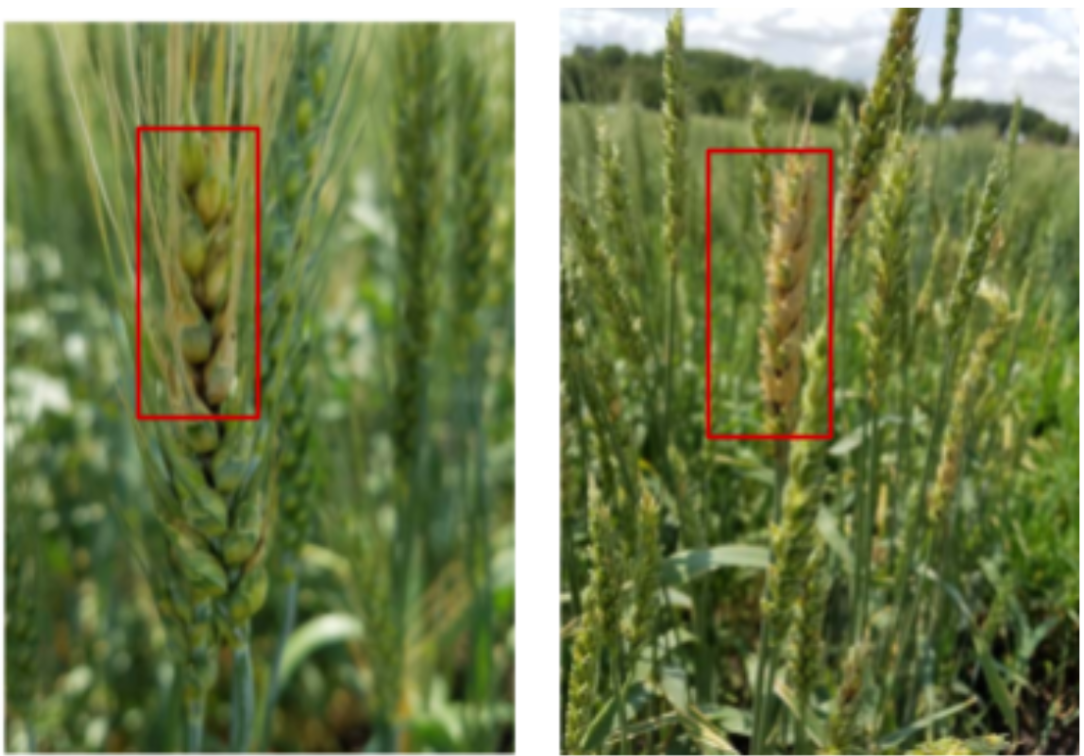
\includegraphics[width=0.5\textwidth]{chapters/chapter2/images/Figure07.png}
    \caption{Symptoms of Fusarium head blight/scab. (A) Early infection signs manifested as a partially bleached wheat head. (B) Advanced infection of Fusarium graminearum \protect\parencite{figueroa2018review}}
    \label{fig:Figure07}
\end{figure}


\subsection{Loose Smut}

Loose smut, caused by Ustilago tritici, replaces wheat spikes with black fungal spores (as observed in Figure~\ref{fig:Figure08}), which are later dispersed by wind. The fungus infects wheat flowers and stays dormant in kernels until germination. It then grows with the plant, destroying floral parts at flowering. The disease thrives in cool, humid conditions and is found wherever wheat is grown. Yield losses depend on infection levels, usually below 1\% but sometimes reaching 30\% \parencite{duveiller2012wheat}.

\begin{figure}[H]
    \centering
    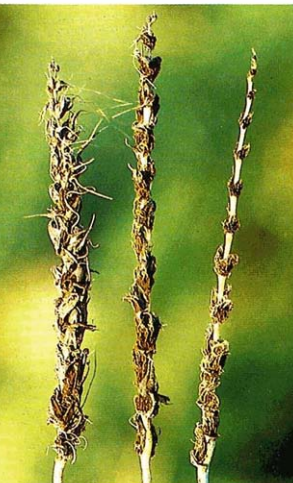
\includegraphics[width=0.6\textwidth]{chapters/chapter2/images/Figure08.png}
    \caption{Loose smut \protect\parencite{duveiller2012wheat}}
    \label{fig:Figure08}
\end{figure}

\subsection{Powdery mildew} 

Powdery mildew (as displayed in Figure~\ref{fig:Figure09}) caused by Blumeria graminis f. sp. tritici affects wheat globally, particularly in cool, dry climates, and can cause yield losses ranging from 10\% to 40\%, with severe cases leading to seedling or tiller death \parencite{singh2023wheat}.

\begin{figure}[H]
    \centering
    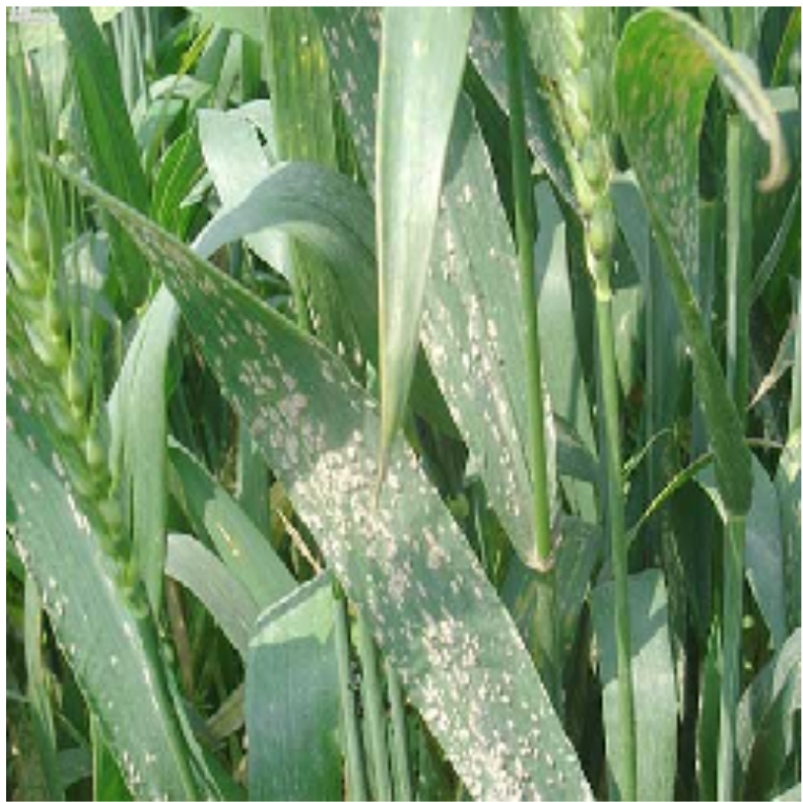
\includegraphics[width=0.4\textwidth]{chapters/chapter2/images/Figure09.png}
    \caption{Powdery mildew from Kaggle dataset ‘Wheat Plant Diseases.'}
    \label{fig:Figure09}
\end{figure}
\subsection{Common Root Rot}

Common root rot, caused by Cochliobolus sativus, Fusarium spp., and Pythium spp., darkens and weakens wheat roots, crowns, and stems (as illustrated by Figure~\ref{fig:Figure10}), sometimes leading to plant lodging and white spikes before maturity. Early infections can cause seedling death.
The disease spreads from infected crop debris, thriving in different soil conditions. sativus in warm, dry soils and Fusarium and Pythium in cool, moist soils. Found in temperate regions, it rarely causes major outbreaks but can lead to localized losses due to reduced plant growth and yield \parencite{duveiller2012wheat}.

\begin{figure}[H]
    \centering
    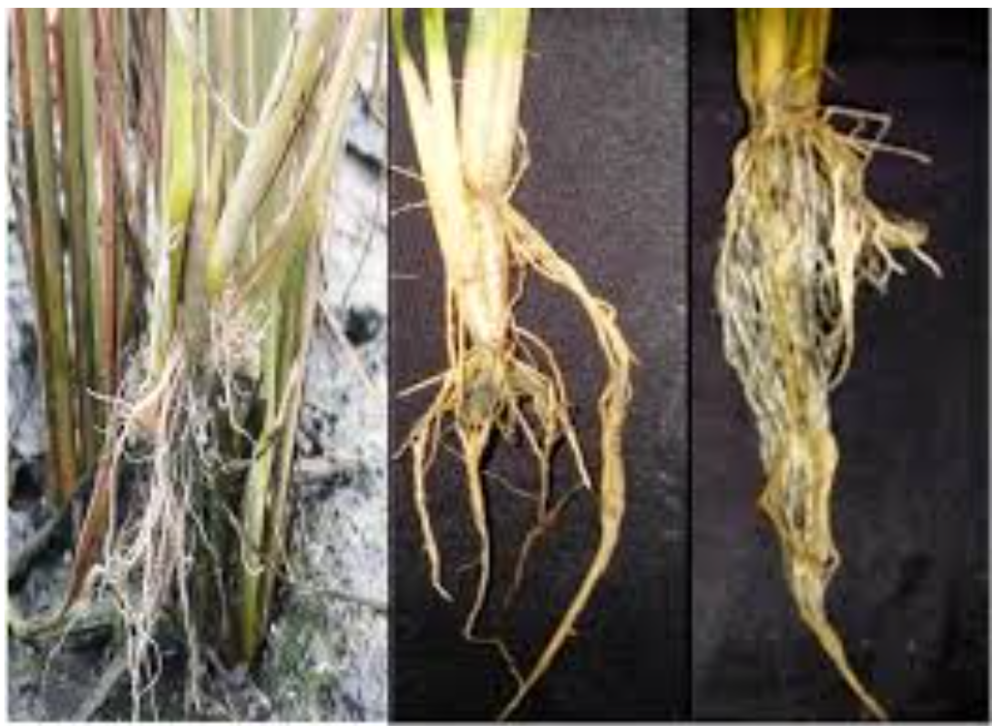
\includegraphics[width=0.4\textwidth]{chapters/chapter2/images/Figure10.png}
    \caption{Common root rot from Kaggle dataset ‘Wheat Plant Diseases.’}
    \label{fig:Figure10}
\end{figure}

\section{Common Insect Pests in Wheat Cultivation}
Wheat is affected by several insect pests that can seriously reduce yield and quality. Below are some of the most common pests and their impacts:

\subsection{Aphids }  
Aphids are nearly transparent, soft bodied sucking insects (as seen in Figure~\ref{fig:Figure11}). When present in sufficient numbers, aphids can cause the yellowing and premature death of leaves. They exude drops of sugary liquid known as “honeydew” \parencite{duveiller2012wheat}.
These pests feed on wheat leaves and grain heads, causing leaf rolling, trapped heads, and poor pollination, particularly during early growth stages. They damage crops by sucking sap from leaves, stems, and kernels, and their honeydew secretion promotes black sooty mold, which hampers photosynthesis and leads to 20-80\% yield losses \parencite{farook2019insect}.

\begin{figure}[H]
    \centering
    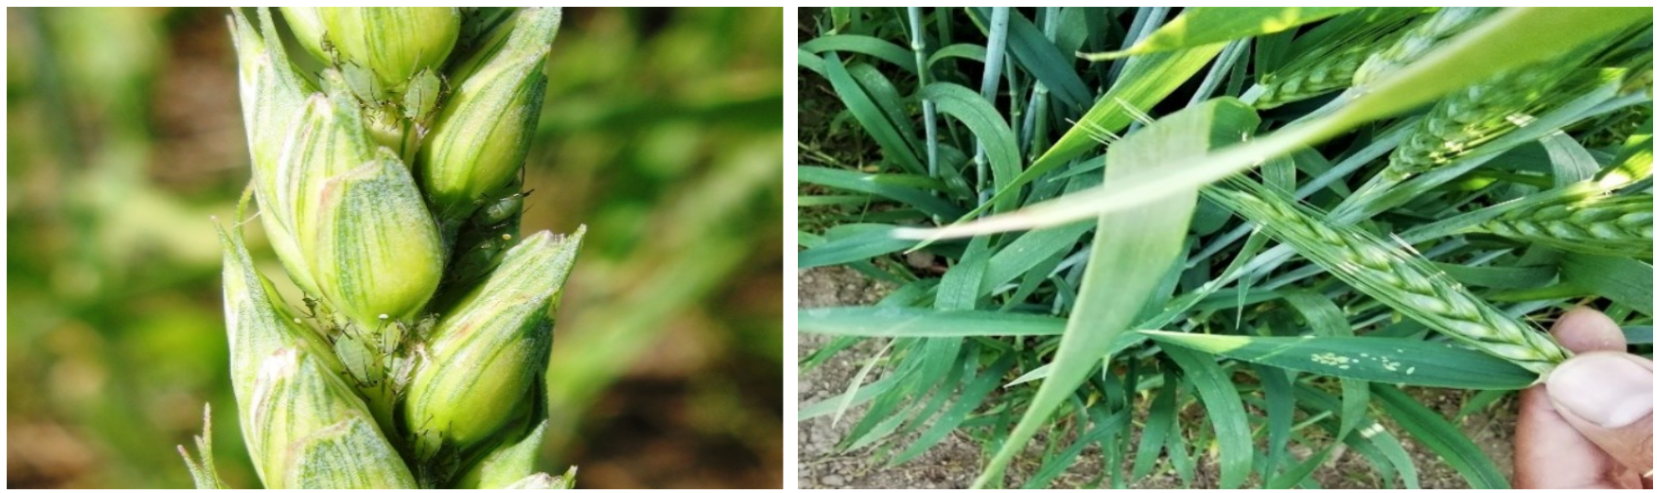
\includegraphics[width=0.6\textwidth]{chapters/chapter2/images/Figure11.png}
    \caption{Aphids on wheat grains (left) and on leaves (right) \protect\parencite{farook2019insect}}
    \label{fig:Figure11}
\end{figure}

\subsection{Cereal leaf beetle}
Adult beetles are 4-5 mm long and have a black head, light brown thorax, and a shiny blue-green wing cover with parallel lines of small dots (as observed in Figure~\ref{fig:Figure12}). Larvae are a dull to bright yellow color but soon take on the appearance of a slimy, globular, black mass due to the mound of fecal material they produce and accumulate on their backs. The most prominent symptom of cereal leaf beetle infestations is the distinct longitudinal stripes on leaves; these stripes are produced by the feeding of adult beetles and of larvae \parencite{duveiller2012wheat}.
Significant yield losses can occur in winter wheat and fall-sown spring wheat. Yield losses of 14\% to more than 25\% have occurred with natural infestations \parencite{duveiller2012wheat}.


\begin{figure}[H]
    \centering
    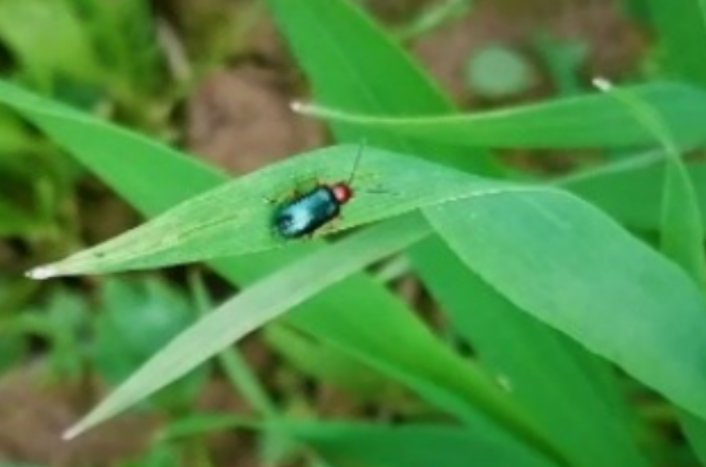
\includegraphics[width=0.6\textwidth]{chapters/chapter2/images/Figure12.png}
    \caption{Adult (left) and larvae (right) of cereal leaf beetle on wheat crop \protect\parencite{farook2019insect}}
    \label{fig:Figure12}
\end{figure}


\subsection{Armyworm}
The armyworm (Mythimna separata Walker) is a pest of wheat. Adult moths are stout and pale brown, while larvae have orange, white, and brown stripes along their sides, a broken stripe on their back, and black spots on the top of their prolegs (as seen in Figure~\ref{fig:Figure13}). Major damage is caused by caterpillars, which move in swarms from field to field, feeding on seedling leaves and ear heads, halting plant growth \parencite{farook2019insect}.

\begin{figure}[H]
    \centering
    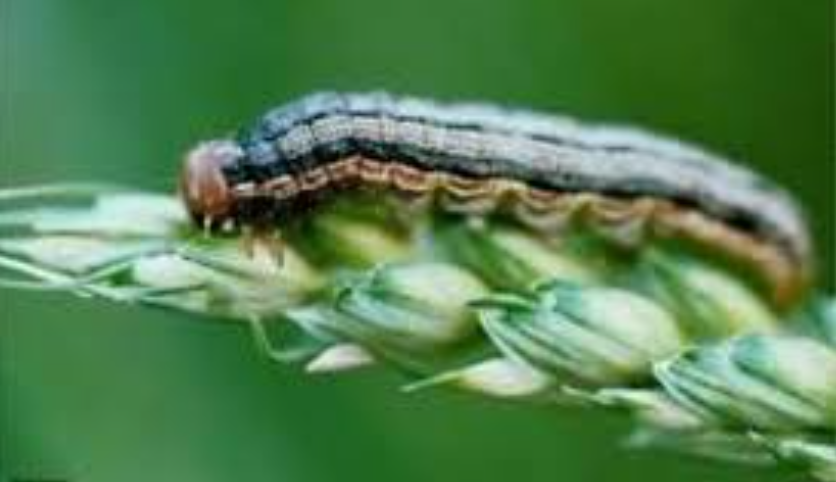
\includegraphics[width=0.6\textwidth]{chapters/chapter2/images/Figure13.png}
    \caption{Armyworm in wheat field \protect\parencite{farook2019insect}}
    \label{fig:Figure13}
\end{figure}

\subsection{Pod Borer}
The pod borer (Helicoverpa armigera) is a polyphagous pest that attacks crops such as gram, lablab, safflower, chilies, groundnut, tobacco, cotton, and wheat. The caterpillars start brown and later turn greenish with dark broken lines on their sides. The adult moth is medium-sized with brownish or greyish forewings featuring a dark crossband and spots, with a wingspan of 3.7 cm (as shown in Figure~\ref{fig:Figure14}) \parencite{farook2019insect}.

\begin{figure}[H]
    \centering
    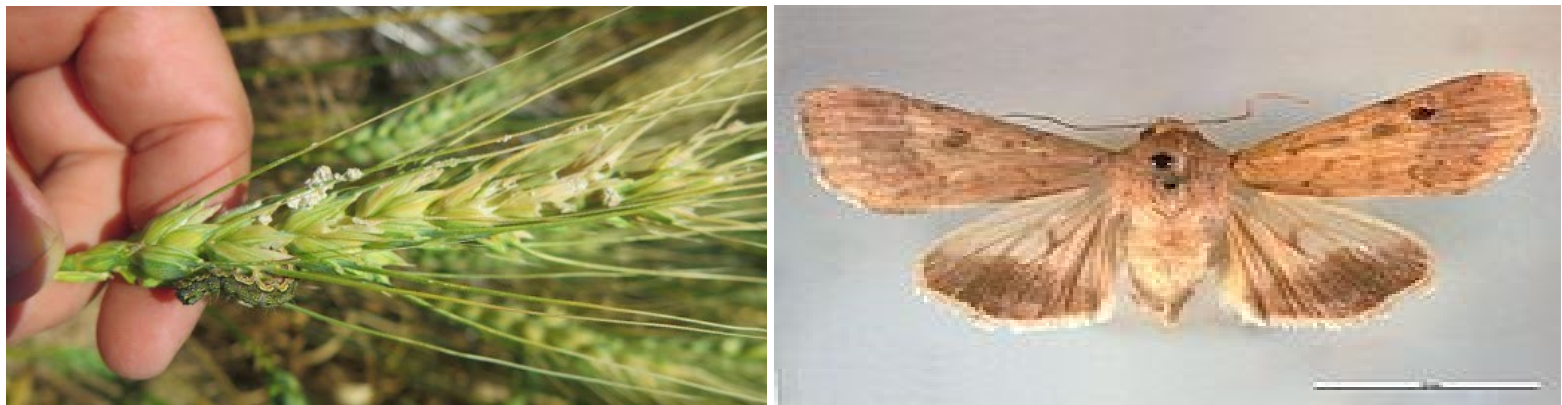
\includegraphics[width=0.6\textwidth]{chapters/chapter2/images/Figure14.png}
    \caption{Pod borer larva (left) and adult (right) from the wheat field \protect\parencite{farook2019insect}}
    \label{fig:Figure14}
\end{figure}

\subsection{Brown wheat mite}  
The brown wheat mite is found in major wheat-growing areas, especially in rainfed conditions. Only females exist and lay two types of eggs in the soil red ones in winter (as seen in Figure~\ref{fig:Figure15}) and white-covered ones in early summer. They damage crops by sucking sap, leading to silvery flecks, yellowing leaves, and reduced grain quality. The mites are active during bright daylight and don’t form webs. Infestation begins in December-January and persists until maturity, with winter rains hindering their multiplication \parencite{kashyap2018identification}.

\begin{figure}[H]
    \centering
    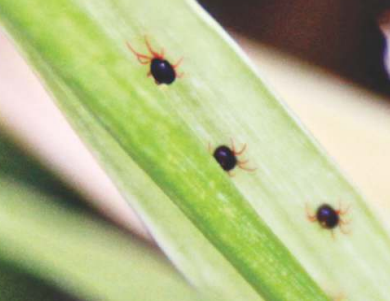
\includegraphics[width=0.4\textwidth]{chapters/chapter2/images/Figure15.png}
    \caption{Brown wheat mite on wheat leaves  \protect\parencite{kashyap2018identification}}
    \label{fig:Figure15}
\end{figure}

\subsection{Pink stem borer}
The pink stem borer (Sesamia inferens), an oriental pest from the Noctuidae family (as illustrated in Figure~\ref{fig:Figure16}), is native to regions such as the Indian subcontinent, China, Pakistan, and Southeast Asia. Initially a rice pest, it has adapted to wheat crops in North-Western India due to changes in tillage practices. Larvae feed inside wheat stems, causing significant damage, including "dead hearts" at the tillering stage and "white heads" at the ripening stage, reducing yields by over 11\% in India. Damage symptoms in wheat are similar to those in rice \parencite{farook2019insect}.

\begin{figure}[H]
    \centering
    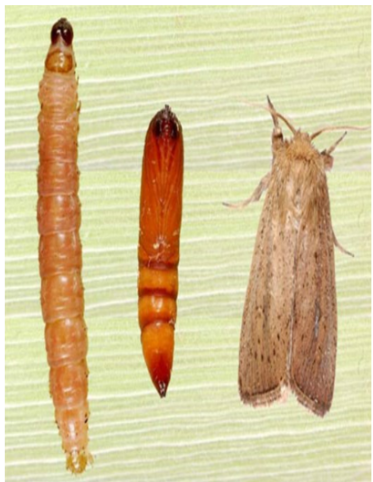
\includegraphics[width=0.3\textwidth]{chapters/chapter2/images/Figure16.png}
    \caption{Pink stem borer  \protect\parencite{farook2019insect}}
    \label{fig:Figure16}
\end{figure}


\subsection{Sawfly} 

Sawflies (as seen in Figure~\ref{fig:Figure17}) produce one generation per year, with larvae overwintering in straw. The legless white larvae bore into wheat stems, weakening plants, causing poor head development, and making them prone to lodging. They primarily target wheat, especially fall-sown varieties, though other cereals can be affected. Infestations are usually patchy and inconsistent. The wheat stem sawfly (Cephus cinctus) is a major concern, it can significantly damage crops. While typically not widespread, sawfly infestations can cause severe localized yield losses \parencite{duveiller2012wheat}.

\begin{figure}[H]
    \centering
    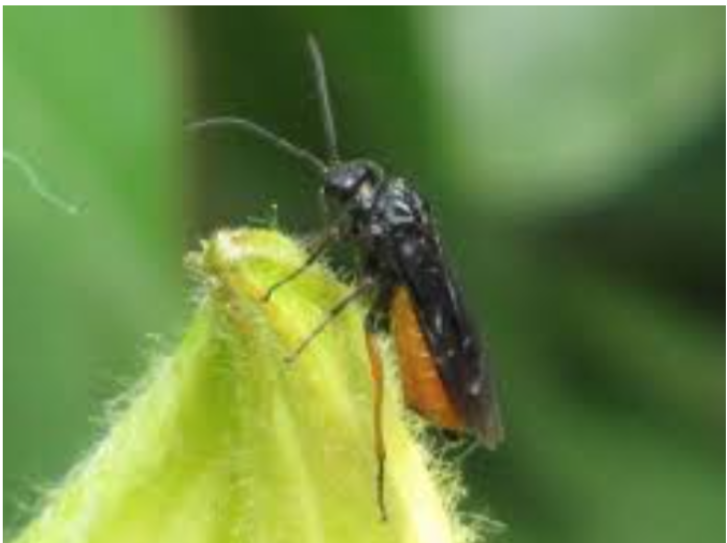
\includegraphics[width=0.4\textwidth]{chapters/chapter2/images/Figure17.png}
    \caption{Sawfly from Kaggle dataset “Pest Dataset.”}
    \label{fig:Figure17}
\end{figure}

\subsection{Slugs, Snails, Grasshoppers, and Crickets}
Slugs, snails, grasshoppers (as referenced in Figure~\ref{fig:Figure18}), and crickets are widespread pests affecting wheat and other plants. They damage crops by chewing leaves, causing a frayed appearance in mature plants. While their presence is often localized, large infestations can significantly impact plant health and yield worldwide \parencite{duveiller2012wheat}.


\begin{figure}[H]
    \centering
    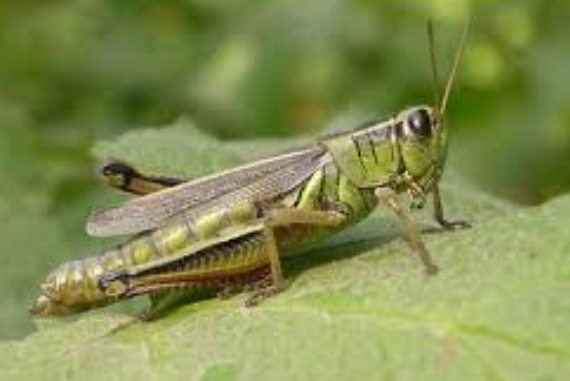
\includegraphics[width=0.4\textwidth]{chapters/chapter2/images/Figure18.png}
    \caption{Grasshoppers from kaggle dataset “Pest Dataset.”}
    \label{fig:Figure18}
\end{figure}

\subsection{Wireworm}
Wireworms are yellow to brown larvae with six short legs (as seen in Figure~\ref{fig:Figure19}). They primarily feed on wheat kernels by consuming the endosperm and leaving only the seed coat. These pests attack young seedlings, often causing "damping off" symptoms and damaging crops at an early stage. Their presence can significantly impact wheat growth and yield, making timely identification and control essential for effective disease management \parencite{farook2019insect}.


\begin{figure}[H]
    \centering
    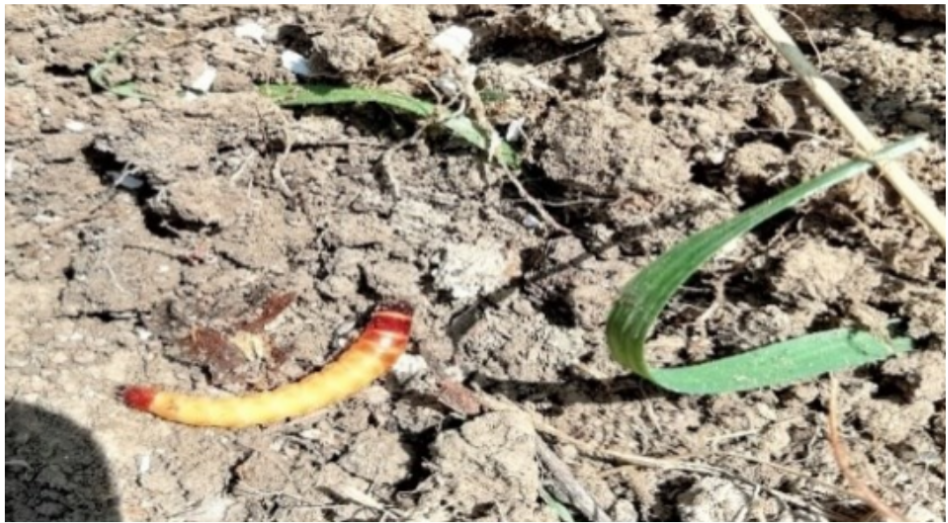
\includegraphics[width=0.6\textwidth]{chapters/chapter2/images/Figure19.png}
    \caption{Wireworm in wheat field \protect\parencite{farook2019insect}}
    \label{fig:Figure19}
\end{figure}


\section{Enhancing Wheat Disease Control Strategies}

Effective wheat disease management combines traditional farming practices with modern technologies. Together, they offer a balanced approach to reducing disease impact and improving crop health.

\subsection{Usual Instruments (Classic Methods)}
These are long-standing approaches that provide the foundation for managing wheat diseases \parencite{mehta2014wheat}. The following practices have been widely used to reduce disease pressure and support healthy crop development.

\begin{itemize}
    \item \textbf{Crop Rotation:} Rotating wheat with non-host crops reduces the buildup of soil-borne pathogens and interrupts disease cycles.
    \item \textbf{Tillage:} Tillage affects disease development by influencing residue decomposition and soil pathogen levels; conservation tillage can increase some necrotrophic diseases.
    \item \textbf{Healthy Seeds:} Clean, pathogen-free seeds minimize seed-borne disease transmission and ensure strong early crop establishment.
    \item \textbf{Soil Management:} Managing soil pH, structure, and nutrient balance helps prevent stress-related susceptibility and supports healthier root systems.
    \item \textbf{Fertilizer Use:} Balanced fertilization strengthens plant defense mechanisms, while over- or under-fertilization can predispose plants to infection.
    \item \textbf{Diversification of Cultivars and Sowing Dates:} Altering cultivars and planting schedules helps reduce the uniformity that pathogens exploit and spreads risk across environments.
    \item \textbf{Use of Resistant Cultivars:} Cultivars bred for specific, partial, or generalized resistance can significantly reduce disease severity, especially when tailored to local pathogen races.
    \item \textbf{Alternative Eco-Friendly Practices:} Methods like field sanitation, residue management, and proper spacing contribute to reducing pathogen survival and disease spread.
\end{itemize}

\subsection{Technological Tools}
Complementing traditional methods, the following tools, rooted in smart agriculture, offer modern solutions to enhance the effectiveness and precision of wheat disease management.

\begin{itemize}
    \item \textbf{Remote Sensing:} Remote sensing using unmanned aerial vehicle-mounted multispectral sensors enables high-resolution monitoring of wheat canopy characteristics across different growth stages. By analyzing spectral bands (Green, Red, Red Edge, Near Infrared), the system captures critical indicators of plant health, canopy structure, and stress conditions, supporting precise and timely crop management \parencite{zhang2025precision}.
    \item \textbf{Disease Forecast Modeling:} Weather-based and biological models are used to predict disease outbreaks and support timely interventions \parencite{mehta2014wheat}.
    \item \textbf{Computer Vision:} Enables automated analysis of crop images for monitoring wheat growth, detecting diseases, and assessing yield. It plays a crucial role in real-time decision-making by processing visual data from the field \parencite{ghazal2024computer}.
    \item \textbf{AI and Machine Learning Algorithms:} Used to interpret complex image data, these algorithms support tasks like disease classification, crop health prediction, and optimizing farm operations by learning from patterns in large agricultural datasets \parencite{ghazal2024computer}.
    \item \textbf{Autonomous Robotic Platforms and Drones:} Facilitate efficient field data collection, spraying, and crop monitoring. These tools reduce manual labor and enable precise, targeted interventions across large wheat fields \parencite{ghazal2024computer}.
    \item \textbf{Precision Agriculture Systems:} Precision agriculture systems integrate technologies like the Global Positioning System (GPS) and the Internet of Things  (IOT) to manage field variability. These technologies help optimize the use of inputs (e.g., water, fertilizer) and support sustainable, data-driven wheat farming \parencite{ghazal2024computer}.
\end{itemize}

\section{Challenges Facing the Integration of Smart Agricultural Systems}
Fully automated smart farming faces both technical and practical challenges. A major obstacle is the generalization of computer vision models across diverse field conditions like lighting, weather, soil, and crop types, which complicates real-time deployment. Robust decision-making in unpredictable outdoor environments also remains difficult, and integrating the full pipeline from image capture to treatment is still under development \parencite{ghazal2024computer}.

On the technical side, communication protocols often support only short distances, limiting scalability. Many devices rely on batteries, reducing operational time. Additionally, processing the large volumes of data generated introduces computational bottlenecks, alongside concerns about privacy, trust, and security in data handling \parencite{idoje2021survey}.



\section{Conclusion}

This chapter presented an overview of the major wheat diseases and pests, along with the current challenges faced in their detection and management. These challenges highlight the need for more advanced and efficient solutions. In the next chapter, we examine how machine learning and deep learning technologies are applied to improve wheat disease classification and pest detection, supporting the shift toward smarter and more sustainable agricultural practices.

